%% LaTeX2e class for student theses
%% sections/evaluation.tex
%% 
%% Karlsruhe Institute of Technology
%% Institute for Program Structures and Data Organization
%% Chair for Software Design and Quality (SDQ)
%%
%% Dr.-Ing. Erik Burger
%% burger@kit.edu
%%
%% Version 1.3.5, 2020-06-26

\chapter{Regression}
\label{ch:Regression}

After extracting features from the elements, the next step is to learn from the data.
The goal of this Bachelor's thesis is to predict the activation barrier of a catalyst molecule.
The techniques used however are not limited to the activation barrier, 
as it can be expected that other properties of the molecule could be predicted with similar techniques.

For regression, artificial neural networks(ANNs) will be used.
Neural networks have seen a huge surge in popularity in recent years for their ability to well
adapt to high dimensional input data.
The concept is derived from biological neural networks such as the ones found in the human brain.

ANNs are a composed of a set of interconnected neurons.
Each neuron has a set of inputs $x_1 .. x_n$, a bias $b$, and an activation function $f(x)$.
The output will be the result of the activation function applied to the sum of all inputs plus the bias.

Neurons are grouped together in layers, where the output of each layer is connected to the input of the next one.
For a single prediction, the example is applied to the input layer, the network is then flooded until the output layer is reached.
In the case of regression used here, the value of the output layer is the prediction of the neural network.

Finding a good performing network architecture is challenging. \\
Since generally no rule is known on what neural network architecture will work best on the given data, the space of possible networks needs to be explored.
A variety of choices for the network architecture can be made, such as the amount of layers, size of the layers, type of activation functions, regularization, normalization, and many more.

When choosing the network architecture, generally a bigger network will be able to adapt to more complex data.
However if the network will become to big, it might encounter issues with overfitting.
Overfitting is a problem encountered when the network adapts to the training data too well.
This will decrease it's ability to generalize the data and make good predictions on previously unseen samples [Figure~\ref{fig:overfitting}].

Measures to counteract overfitting include regularization and dropout layers.
Regularization introduces a penalty term that punishes the network for extreme values.
This causes the network to adapt less well to the training data, but in return can help with the network
performance on previously unseen data.

Dropout layers randomly disable neurons in a layer.
This forces the network to be less reliant on certain neurons, and instead learn the data in the entire network.
\\

To find a suitable network architecture, a hyperparameter optimization needs to be performed.
Hyperparameter optimization aims to find a good performing network architecture by testing the performance
of different networks on the data.
%TODO: Mehr?

\begin{figure} [h]
    \centering
    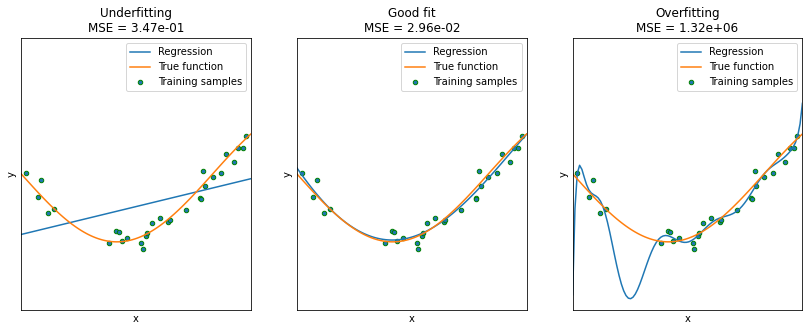
\includegraphics[width=0.9\textwidth]{figures/regression/overfitting.png} 
    \caption[Overfitting]{Regression on a function with training examples. 
            The underfitting model is not complex enough to fit to the data well. 
            The overfitting model is too complex for the data.
            While the training error is lower for the overfitting model, 
            the overall performance of the overfitting model on previously unseen data 
            is worse than for the model with a good fit.
        }
    \label{fig:overfitting}
\end{figure}
  
To prevent overfitting while still getting good regression results, multiple network architectures need to be considered.
The networks proposed here were found by a manual exploration of the network architecture first.
In a second step, hyperparameter analysis was run to find a good network architecture.

\paragraph{Technicalities}

All networks were generated in Keras, an open-source deep learning library.
Keras offers a high level Python API to create, train and analyse neural networks.

To allow for better training and predictions, all features and labels were standardized before being passed to the neural network.
Standardizing is a process where each feature $f$ is scaled to independently so the mean over all samples in the dataset is 0, 
and the every feature has unit variance.
This can easily be achieved by independently subtracting the mean $\overline{f}$ over all samples, and dividing by the standard deviation $\sigma_f$.

$$
f_{norm} = \frac{f- \overline{f}}{\sigma_f}
$$

The same scaling is applied to the labels.
This means the networks do not directly predict the activation barrier, but the networks prediction needs to be scaled back first.

Hyperparameter optimization was performed using keras-tuner, a hyperparameter tuner for Keras.
Keras-tuner offers a variety of different algorithms.
In the hyperparameter optimizations performed here, Keras Hyperband was used.
Keras Hyperband is an  implementation of the Hyperband algorithm propsed in \cite{li2017hyperband}.
It focuses on an optimized search speed compared to other Hyperparameter optimization methods, such as
Bayesian Optimization, by adaptive resource allocation and early stopping.

Hyperparameter optimization took multiple hours for LEFD features, 
and multiple days for SNAP features.
Training and hyperparameter optimization was performed on the universtiy cluster %TODO: Notwendig?
using a Nvidia Tesla V100-SXM2-32GBa GPU.

During training and hyperparameter optimization, a fraction of the data was reserved as test set.
This test set was not used for training or validation, but only to evaluate the final performance of the networks.
All data about network performance in this chapter is measured on the test set, unless specified otherwise.

During training of a network it is common practice to reserve a validation split that is not used to train the network.
Instead, the networks performance while training is measured on the validation data, and tuned to achieve similar accuracies on
training and validation data.
This helps to avoid overfitting in the network, since the network can no longer just memorize the training
data, but instead has to achieve good performance on data not seen during training as well.

This means there is a total of 3 datasets, one being used for training, the other being used to validate the networks
performance during and after training, and the last being used after hyperparameter optimization to evaluate the final network
performance.

\section{Regression on fourier descriptor features}
\label{sec:Evaluation:fourier}

In the first approach, the features generated by the fourier descriptor were used.
Notable hyperparameters to the feature extractor here are the number of layers $l$ and the order $o$ of the fourier descriptor.

The start and end height of the layers are chosen so that all the molecules in the dataset fully fit within $z_{min}$ and $z_{max}$.

The output shape of the descriptor will be an array of size $l \times (o * 4 - 1)$.
Generally, the bigger the number of fourier coefficients, the better the contour can be approximated.
However, an order that is chosen too high may increase the risk of overfitting.

The highest accuracy of prediction is not the only metric to be considered when choosing these hyperparameters.
Since the ultimate goal is not to get the most accurate prediction possible, but instead discover which parts of 3D space 
are responsible for prediction, an order that offers reasonable high accuracy of prediction and 
allows for an interpretation of the feature space needs to be found.

After various tests with multiple orders, an order of $k_{max} = 10$ seemed to be a good compromise between accuracy of description and accuracy of prediction.
The following results will be focused on an order of $10$.

The same problem is faced when defining the number of slices.
Here the problem becomes more tricky, since the number of slices seems to play a huge part in the architecture of the ANN used.
This means hyperparameter analysis needs to be performed individually for every choice of the number of layers.

Since every slice is composed of same kind of fourier coefficients, the first idea was to use convolution layers to decrease the dimensionality of the input.
Filters might be able to recognize structures in each of the slices, and applied them across the different slices.

Convolution layers heavily depend on the assumption that the relative location of the features matters.
Filter sizes were therefore chosen to correspond to the dimensions over which similarities in the structures of the features are expected.
In the case of fourier coefficients, the filter therefore were only stretched along the dimension of the different $z$ layers, and not along the dimension of the fourier descriptors.

Multiple tests were performed with various filter sizes and convolution layers.
The regression accuracy was falling short of expectations, and the general shape of the convolution part of the network did not seem to change the prediction accuracy significantly.

\begin{figure} [h]
    \centering
    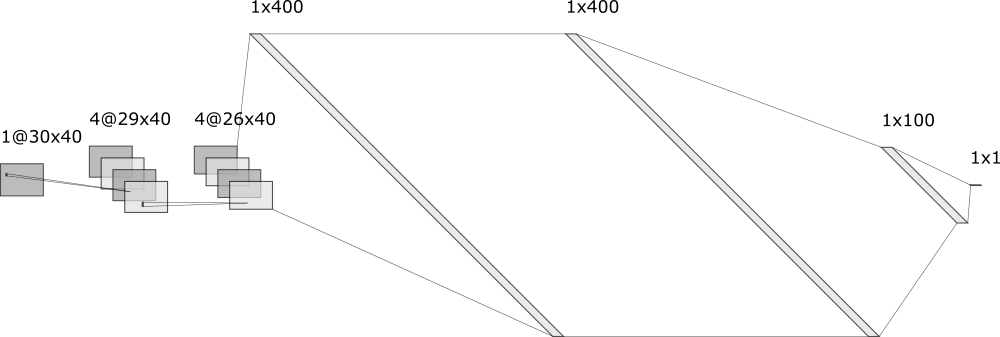
\includegraphics[width=0.7\textwidth]{figures/regression/fourier/cnn/fourier_conv_layout.png} 
    \caption[Layout of LEFD CNN]{
        Architecture of the convolutional neural network used for predicting the activation barrier from fourier coefficients.
    }
    \label{fig:cnn-architecture}
\end{figure}

In first network architectures, overfitting was a mayor problem.
With regularization and other techniques the issue of overfitting could be reduced.
What became clear pretty early in the tests was that convolution layers did not improve prediction accuracy as expected.
When testing different filter configurations, the network performed best the smaller the filters got, and the fewer convolution layers were used.
In the end, the best performing convolutional neural network found had two convolution steps with a filter size of $2 \times 1$ for the first layer, and a filter size
of $4 \times 1$ for the second layer [Figure~\ref{fig:cnn-architecture}].
After the convolution layers 3 fully connected layers and the output layer followed.
Dropout and batch normalization layers were added in between to reduce overfitting.
The prediction accuracy of the CNN was similar yet slightly worse than the prediction accuracy achieved on autocorrelation features \cite{friederich_dos}.
The best CNN achieved a mean squared error over all test examples of $MAE=1.36 kcal/mol$ and a coefficient of determination of $r^2=0.84$ \ref{fig:fourier_cnn} when trained on a train fraction of 80\%.
In comparison, the best neural network of \cite{friederich_dos} achieved a prediction accuracy of $MAE=1.12 kcal/mol$ and $r^2=0.845$.

Since the space of possible network configurations is highly irregular, there is likely a network configuration using convolution layers 
that performs better than the one found here.
However all the tests performed were indicating that densely connected layers would achieve similar or higher accuracy.
The idea of convolution layers was therefore dropped early on, and instead the focus was shifted to optimizing a fully-connected architecture.
\\ 

\begin{figure}[!htb]
    \minipage{0.1\textwidth}
    \endminipage\hfill
    \minipage{0.4\textwidth}
      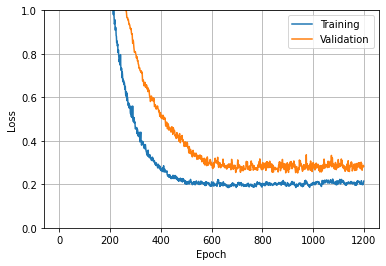
\includegraphics[width=1.0\textwidth]{figures/regression/fourier/cnn/lossCNN.png}
    \endminipage\hfill
    \minipage{0.4\textwidth}
      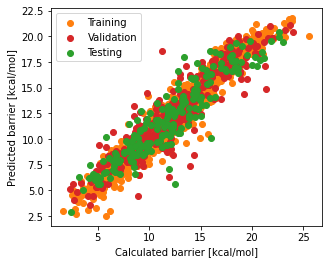
\includegraphics[width=1.0\textwidth]{figures/regression/fourier/cnn/scatterCNN.png}
    \endminipage\hfill
    \minipage{0.1\textwidth}
    \endminipage
    \caption[CNN trained on LEFD features]{
        Loss while training the CNN. The jitter in the training loss during convergence is likely caused by the dropout layers. 
        The optimization goal was minimizing the mean squared error. 
        Training was performed on 80\% of the data.
        On the right are the predictions of the activation barrier in comparison to the real values ($MAE=1.36$, $r^2=0.84$).
    }
    \label{fig:fourier_cnn}
\end{figure}

Since \cite{friederich_dos} has shown that similar accuracy to the convolution approach can be achieved by learning from autocorrelation features,
the next idea was to use a transfer learning approach.
In a first step, the network was trained to predict the autocorrelation features computed in \cite{friederich_dos}.
In a second step, the network is then extended with additional layers to learn to predict the activation barrier [Figure~\ref{fig:transferlearn}].
The hope was that teaching the network about autocorrelation features, the model would learn to recognize relevant properties of a catalyst.
In a second step, the entire network would then be trained to adapt specifically to the activation barrier.

\begin{figure} [h]
    \centering
    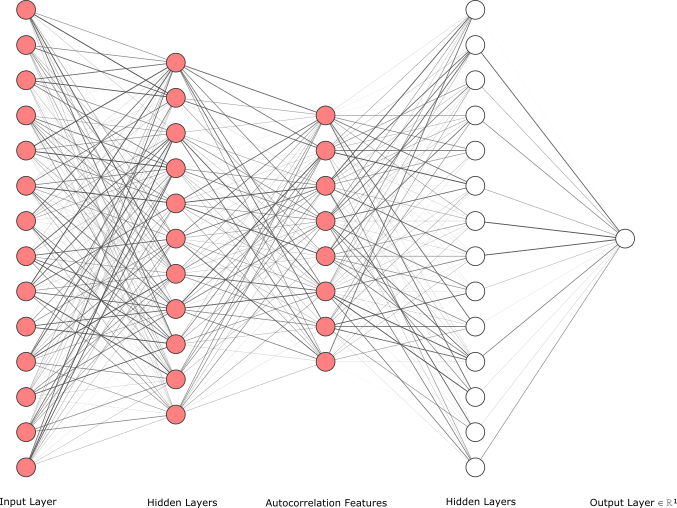
\includegraphics[width=0.7\textwidth]{figures/regression/fourier/nn.png} 
    \caption[Transfer learning model]{Illustration of the transfer learning approach.
        In red the original model predicting autocorrelation features from the input is illustrated.
        In white the second part of the network, predicting the activation barrier from the autocorrelation features, is illustrated.
        Different sizes and amounts of hidden layers were tested. Here, single hidden layers are shown for illustration purposes.
    }
    \label{fig:transferlearn}
\end{figure}

Since the convolutional approach did not seem to improve results, a fully connected architecture predicting autocorrelation features from fourier coefficients 
was used.
Since there were 30 autocorrelation features used, the last layer of the network had a size of 30.
Findings about good hyperparameter, such as layer size, regularization and dropout rates, could be partly reused from the convolution step.
In the end, a network that predicted the 30 independent autocorrelation features was found.
The network was able to predict some autocorrelation with very high accuracy. Specifically, the $T$ features and $I$ features were
predicted with an accuracy of $r^2 > 0.98$. 
Other features, such as $Z$ features, were lacking behind in accuracy, with the network only being able to reach accuracy of $r^2<0.96$ for some features.
The features the network was able to approximate well were also less important to the network found in \cite{friederich_dos}, while the features 
the network performed poorly on were the more important features \ref{fig:transfer_result}.

\begin{figure}[h]
    \minipage{0.32\textwidth}
      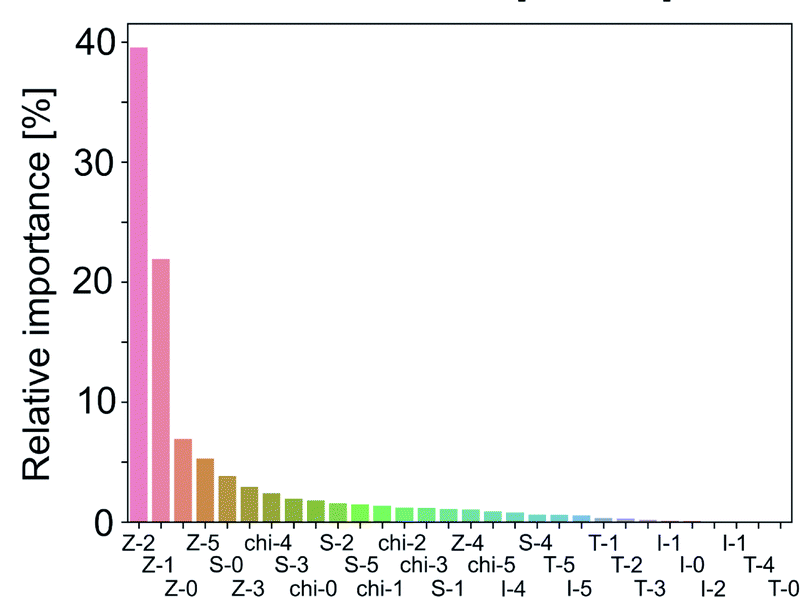
\includegraphics[width=1.0\textwidth]{figures/regression/fourier/importance_map.png}
    \endminipage\hfill
    \minipage{0.32\textwidth}
      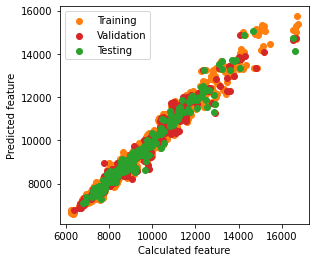
\includegraphics[width=1.0\textwidth]{figures/regression/fourier/transfer/scatterZ2.png}
    \endminipage
    \minipage{0.32\textwidth}
      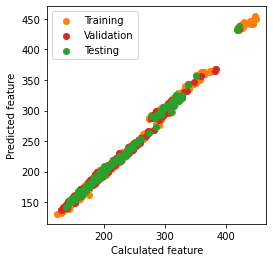
\includegraphics[width=1.0\textwidth]{figures/regression/fourier/transfer/scatterT0.png}
    \endminipage
    \caption[Prediction of autocorrelation features from LEFD]{
    Importance of features for the neural networks (left). Reprinted from \cite{friederich_dos}.
    Prediction of Z-2 features from fourier features (middle) and prediction of T-0 features from fourier features (right). 
    The network was trained on a train fraction of 80\%.
    }
    \label{fig:transfer_result}
\end{figure}

After the network predicting the autocorrelation features was trained, the transfer learning was started.
The last layers of model were removed, and replaced with newly initialized layers.
These newly added layers have an output size of 1 to allow for prediction of the activation barrier.
The best configuration found kept the first 3 layers of the original network, and then added 3 additional hidden layers and one output layer.
Regularization and normalization was used for some of the layers.
The model was then trained again with fourier coefficients as input and activation barriers as output.
Compared the convolution approach, the network took longer to converge and overall regression accuracy improved.
The network achieved a $r^2=0.874$ and a $MAE=1.139 kcal/mol$ when trained on 80\% of the data Figure~\ref{fig:transfer_final}.

\begin{figure}[!htb]
    \minipage{0.3333\textwidth}
      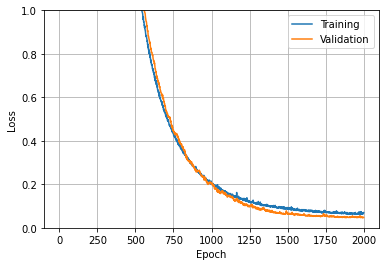
\includegraphics[width=1.0\textwidth]{figures/regression/fourier/transfer/lossTransferAutocor.png}
    \endminipage\hfill
    \minipage{0.3333\textwidth}
      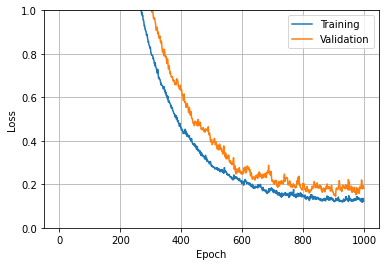
\includegraphics[width=1.0\textwidth]{figures/regression/fourier/transfer/lossTransferFull.png}
    \endminipage\hfill
    \minipage{0.3333\textwidth}
      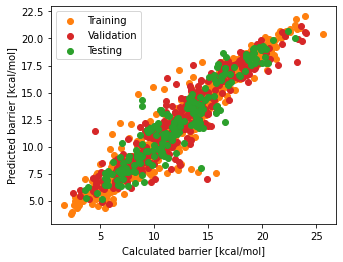
\includegraphics[width=1.0\textwidth]{figures/regression/fourier/transfer/scatterTransferFull.png}
    \endminipage
    \caption[LEFD transfer learning]{
    Loss of the network being trained to predict autocorrelation features (right).
    The adapted network is then trained again to predict the activation barrier. The loss function in the middle shows the second training.
    The prediction accuracy has slight improved (right).  
    Both networks are trained on a train fraction of 80\%.
    }
    \label{fig:transfer_final}
\end{figure}

In an attempt to find a better network architecture, a hyperparameter optimization was performed.
Hyperparameter optimization is a way of finding good hyperparameter for the underlying problem.
A searchspace need to be defined manually first, an optimization algorithm is then run to find good parameters within the search space.
Generally a bigger search space mean longer computation time for the hyperparameter algorithm.
The search space here was limited by the findings of manual hyperparamter tuning.
Notable optimization values given to the hyperparamter tuner were the number and size of fully connected layers, the regularization rate of these layers, and the dropout rate for the layers.
The optimizer also had control over the learning rate.

\begin{figure}[!htb]
    \minipage{0.3333\textwidth}
      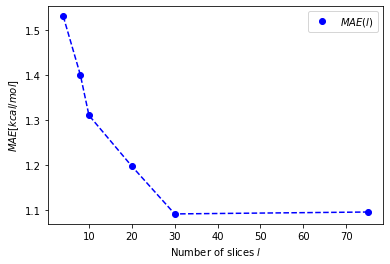
\includegraphics[width=1.0\textwidth]{figures/regression/fourier/mae_layer.png}
    \endminipage\hfill
    \minipage{0.3333\textwidth}
      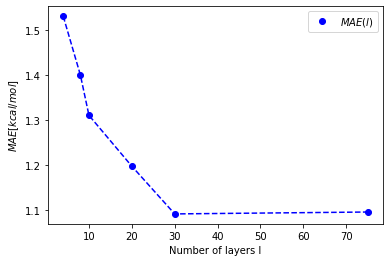
\includegraphics[width=1.0\textwidth]{figures/regression/fourier/r2_layer.png}
    \endminipage\hfill
    \minipage{0.3333\textwidth}
      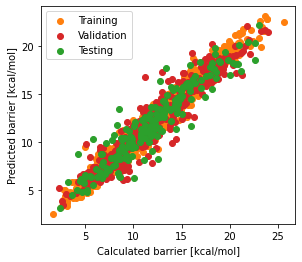
\includegraphics[width=1.0\textwidth]{figures/regression/fourier/scatterHyperparam.png}
    \endminipage
    \caption[Evaluation of LEFD models]{
    The $r^2$ values and $MAE$ for different layer heights.
    For all layer heights a separate hyperparameter optimization wa run, resulting in different network architectures.
    All networks are trained using 80\% on the data. The $r^2$ scores and $MAE$ were evaluated later using a test dataset.
    On the right the prediction of the best performing network found in the hyperparameter optimization step is plotted.
    }
    \label{fig:fourier_final}
\end{figure}


In addition, multiple hyperparameter optimizations were performed for different layer heights $l$.
Since the layer heigh also changes the input size of the neural network, an assumption about the 
architecture across different layer heights is not feasible.
For ever layer height a separate hyperparamter optimization was run [Figure~\ref{fig:fourier_final}].
The best hyperparameters found for every input size vary substantially.
The best network achieved an accuracy of $MAE=1.096 kcal/mol$ and $r^2=0.882$ on a training fraction of 80\%.
It was trained on features generated from a layer height of $0.2$, resulting in a total of $75$ layers.

After a certain layer height the prediction accuracy seems to no longer improve.
The step from 30 to 75 layers does not change the accuracy significancy, while more than doubling input size.
The improvement in accuracy from 30 to 75 layers is so small that it might be an artifact of the 
randomness of training, and does not necessarily mean that the network is able to learn better from the higher amount of layers.

The process shows that performing regression on fourier features is possible.
The accuracy however is worse than other machine learning techniques on autocorrelation features, especially when trained on small training fractions.
Since the goal of this thesis is to learn from the 3D structure of the molecule, the similar performance to networks trained on autocorrelation features
might indicate that the information learned from the 3D structure is limited.
This assumption is further validated by the fact that the transfer learning approach that 
tries to eliminate spacial information about the element in the middle of the network, achieves similar accuracy to the 
network trained on features that do not include any information about the 3D structure.

In an effort to improve prediction accuracy, a different feature extractor, SNAP, was developed.

\section{Regression on SNAP features}
\label{sec:Evaluation:snap}

Similar to the feature space for fourier coefficients, the shape of the SNAP feature space is determined by two factors.
The first is the number of different species in the dataset.
The second is the resolution of the encoding defined by $n_{max}$ and $l_{max}$.

Other hyperparameters, such as the choice of radial basis functions, might influence the prediction accuracy further.

The number of radial basis functions $n_{max}$ and the maximum degree of spherical harmonics $l_{max}$ do both influence
the input dimension.
The ideal network architecture for different values will depend on the choice of these values.
The higher the degree of the spherical harmonics and radial basis functions, the more precise the element can be described. %TODO: The element or the space?
The choice of $n_{max}$ and $l_{max}$ will also determine the accuracy when trying to interpret the predictions of the model later on.

Hyperparameter analysis was performed on different combinations of $n_{max}$, $l_{max}$.
Since hyperparameter optimization is very computationally expensive, taking up to multiple days on modern high-performance 
server hardware, the number of combinations that could be explored is limited.

SNAP features are not fully rotationally invariant.
In order to allow the model to learn about the different possible rotations of the molecule, data augmentation was used.

During the first hyperparameter optimizations, 20 evenly spaced rotations of the molecule along the $z$-Axis were used.
The features for all of the 20 rotations was then fed into the model.
Tests with different augmentation steps showed that 20 augmentations seemed to be a good balance between 
accuracy and training speed.
Since the size of training examples rises linearly with the number of data augmentations,
high numbers of augmentations will drastically decrease training speeds.
This will in effect also reduce the speed of hyperparameter optimization.

\subsection{Convolution neural network}

Similar to the features generated by LEFD, the output of SNAP can be shaped into a feature matrix again.
Here, each layer will correspond to one species of atoms.
Since the dataset the model is trained on consists of 12 different species of atoms, the feature matrix will have a height of 12.
Each row will then contain the coefficients describing the density of one species around the iridium center.
Depending on the choice of $n_{max}$ and $l_{max}$, the number of coefficients for each species will change.

Since a coefficient of the $k$-th row will correspond to $c^k_{nlm}$, meaning every coefficient in the same colum has the same spacial meaning just for a different species,
a convolutional neural network was the first idea to reduce the size of the input space and allow the network to learn structure in the input data.

Not every species of atoms is present in every molecule, which means the input matrix will generally be sparse.
Rows that correspond to atoms not in the molecule will be filled with 0.
A filter that learns the general structure of the space and that is moved over the different species, therefore 
being able to ignore sparse inputs seemed to be a good choice.

Using a hyperparameter optimization to find the ideal filter size and number of convolution layers however showed
the a fully connected approach reaches higher accuracy than convolutional layers.
The hyperparameter optimizer not only gravitated towards a small amount of filters, but also towards 
the smallest possible filter size allowed in the hyperparameter space.

In further optimization the idea of convolution layers was therefore dropped in favour of fully connected layers.

If in the future the $n_{max}$ and $l_{max}$ parameters or the number of species are increased drastically, 
convolutional layers might become relevant again.

\subsection{Fully connected neural network}

In a next step, hyperparameter optimization was focused on fully connected layers.
For different combinations of $n_{max}$ and $l_{max}$ hyperparameter optimizations were run.

The hyperparameter optimizer was allowed to choose between 1 to 8 fully connected hidden layers.
For each layer, the number of neurons, regularization rate and dropout rate could be chosen by the optimizer.
Additionally, the optimizer had the option to add a batch normalization layer after each of the fully connected layers.
The layers were then finished off with one neuron fully connected to the last hidden layer.

The activation function for each of the layer was fixed to Relu activations.

Using the Hyperband Optimizer, the configurations discussed in the following sections were found.

\paragraph{Feature size}
The expectation was that the more accurate the density space would be described, the higher the prediction accuracy would be.
However after a full hyperparameter optimization on a variety of combinations of $n_{max}$ and $l_{max}$,
the differences in accuracy were not as significant as expected.
While increasing the number of $n_{max}$ coefficients seemed to increase the prediction accuracy,
increasing the number of spherical harmonics $l_{max}$ did not play a significant role in prediction accuracy [Figure~\ref{fig:snap_hyperparameter}].
Highest prediction accuracies where achieved by networks performing regression on features generated with $n_{max} > 6$.

The interpretation here is that distance to the metal center plays an important role to predicting the activation
barriers in the dataset, while the location seems to be less important.

Since hyperparameter searches for are very costly, hyperparameter analysis was run to an $n_{max} = 9$.
Significantly increasing $n_{max}$ might further improve prediction accuracy.

\begin{figure}[!htb]
  \minipage{0.3333\textwidth}
    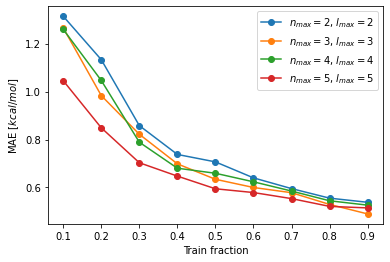
\includegraphics[width=1.0\textwidth]{figures/regression/snap/fixnl.png}
  \endminipage\hfill
  \minipage{0.3333\textwidth}
    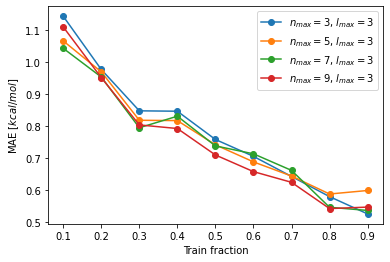
\includegraphics[width=1.0\textwidth]{figures/regression/snap/fixl.png}
  \endminipage\hfill
  \minipage{0.3333\textwidth}
    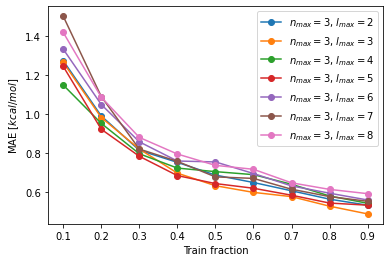
\includegraphics[width=1.0\textwidth]{figures/regression/snap/fixn.png}
  \endminipage
  \caption[Learning curves for different SNAP resolutions]{
  Networks for SNAP features trained on different train fractions.
  All networks were trained on the hyperparameters found for the corresponding $n_{max}$ and $l_{max}$.
  $|v|$ is the size of the feature vector.
  Networks were trained with 10 data augmentation steps and a cutoff radius of $12 \AA$.
  Hyperparameter search was run on a training split of 80\%.
  }
  \label{fig:snap_hyperparameter}
\end{figure}

\paragraph{Cutoff sphere}
All hyperparameter searches were run with with a cutoff radius $r_{cut} = 20 \AA$.
This cutoff sphere is large enough to fully fit every element of the dataset into it.
However, due to the nature of the radial basis functions used, the resolution of atoms 
further away from the center will decrease.
To test the influence of the cutoff radius on the prediction, 
networks were trained on features generated with different cutoff radii.
The network architecture was based on the hyperparameter optimization performed earlier.

For every configuration of $n_{max}$ and $l_{max}$, a networks were trained for a variety 
of tests splits and data augmentation steps.
These networks were then evaluated by their performance with respect to the cutoff radius.

Up to a cutoff radius of $8 \AA$, the mean network performance improved. 
At a training fraction of 80\%, the mean classification error among 
all networks decreased from $0.588 kcal/mol$ for a cutoff radius of $4 \AA$ to 
$0.558 kcal/mol$ for a cutoff radius of $8 \AA$.
From there however, increasing the cutoff radius did not improve the accuracy further.
Instead, the mean MAE increased again.
This lead to the hypothesis that atoms closer to the metal center are more important to the activation barrier than atoms further away from the center.
This hypothesis could also explain the slight increase in prediction error when further increasing the cutoff radius.
Since the resolution of the feature space is limited, increasing the cutoff radius will decrease the accuracy 
with which the inner atoms are described in the features, which might have caused a decrease in prediction accuracy.

To verify this hypothesis, a second experiment was run.
Here, all atoms outside a cutoff sphere were removed from the element before passing it on to the encoder,
while the radius $r_{cut}$ of remained untouched at $r_{cut}=12$.
The networks were once again trained with the hyperparameters found in the initial hyperparameter analysis.
The training was run for cutoff spheres with radius $r_{del} \in 2\AA, 4\AA, 6\AA, 8\AA$.
For $r_{del}=2$, no prediction was possible and the networks just predicted the mean of the data.
This was to be expected since at this cutoff radius, only $5.4\%$ of the elements are encoded into the features.
However for $r_{del}=6$ the mean MAE over all networks trained on 80\% of the data was at $MAE = 0.732 kcal/mol$. 
For $r_{del} = 6$ 95\% of the atoms are included in the data. 
The remaining 4\% fall outside of the cutoff sphere and are ignored. 

For $r_{cut}=8$ the mean MAE over all networks trained on 80\% of the data was at $MAE = 0.734 kcal/mol$. 
At this cutoff radius, 100\% of the atoms are included in the data.
This accuracy is within the margin of error that could be caused by the randomness of the training process
indicating that the prediction accuracy for $r_{del} = 6$ and $r_{del} = 8$ are virtually identical.

This lead to the conclusion that atoms close to the center seem to be more important to the activation barrier than 
elements further away.
This could however just be caused by the fact that atoms very far from the center tend to be hydrogen and carbon 
atoms which are believed to play a less significant role in the activation barrier than other elements.
When examining multiple $r_{cut}$ values, choosing a tight $r_{cut}$ achieves the best prediction accuracies.
Looking at the nature of the encoding, this intuition is verified.
Empty space that is indirectly included into the encoders features.
Since the encoder will try to encode a density of 0 in these regions,
the features need to be chosen accordingly.
This means the features to encode empty space will compete with the features encoding
actual information about the molecule.
The less empty space needs to be encoded, the more accurate actual density can be represented.
From now on, all cutoff radii will therefore be chosen at $r_{cut} = 8 \AA$.

\begin{figure}[!htb]
  \minipage{0.3333\textwidth}
    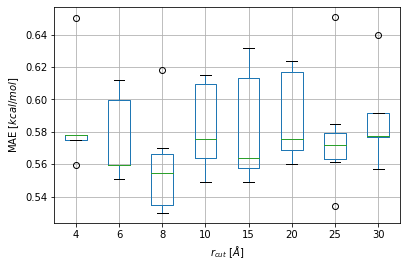
\includegraphics[width=1.0\textwidth]{figures/regression/snap/rcut-compare.png} %TODO: REPLACE!!!!
  \endminipage\hfill
  \minipage{0.3333\textwidth}
    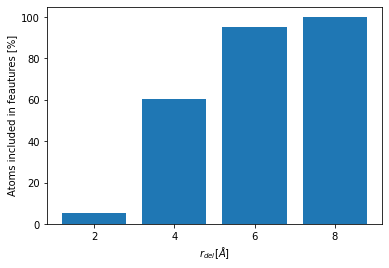
\includegraphics[width=1.0\textwidth]{figures/regression/snap/cut-sphere-perc.png}
  \endminipage\hfill
  \minipage{0.3333\textwidth}
    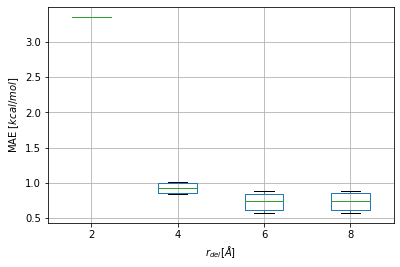
\includegraphics[width=1.0\textwidth]{figures/regression/snap/cut-sphere-comp.png}
  \endminipage\hfill
  \caption[Comparison of SNAP cutoff radii]{
  On the left are networks with different $n_{max}, l_{max}$ trained on different cutoff radii.
  On the right are networks trained with a cutoff sphere $r_{del}$ outside of which all atoms are removed and a fixed $r_{cut} = 12 \AA$.
  The center shows the percentage of atoms included in the cutoff sphere with radius $r_{del}$.
  All networks are trained on a train fraction of 80\%.
 }
  \label{fig:snap_hyperparameter}
\end{figure}


\paragraph{Sensitivity to rotation}
Since SNAP features are not fully rotationally invariant, the networks ability to abstract rotation from the input is crucial.
In order to teach the network about the possible rotations of an element, 
the element is augmented by rotating it around the remaining axis of freedom, the $z$ axis.
For every augmentation step, the rotated element is added to the training data.
Tests with different augmentation steps were performed.
All networks were trained on the previously found hyperparameters.
The augmentation steps ranged from 5 evenly spaced rotations to 100 evenly spaced rotations.
Both the training and the test data was augmented to allow for learning from the augmented data
as well as to validate if the network was actually able to abstract away rotations.

Even with only 5 data augmentation steps the networks achieved a mean prediction error of $MAE = 0.584 kcal/mol$ trained on 80\% of the data.
The mean error over all networks decreased up to 30 augmentation steps.
After 30 augmentation steps no further decrease in mean prediction error was observed.
For networks with higher data augmentation steps, the stability of the networks when trained on small train splits was higher.

When looking a networks prediction over 360 different rotations, networks trained with higher data augmentation 
are significantly more stable to rotation than networks trained on a smaller number of of rotations [Figure~\ref{fig:snap_roation}].
When comparing a network trained on 20 rotations to a network trained on just 5 rotations,
the difference becomes clear.
For the network trained on 5 rotations the prediction accuracy very accurate for rotations included in the training data.
For rotations not in the training data, the prediction diverges significantly, indicating the inability of the network to abstract away rotation.

For the network trained on 20 rotations, the divergence is very limited.
However in some cases, while the overall prediction accuracy is decreased for the network trained on 
more data augmentations, the accuracy for some rotations is more precise on the network trained on a lower number of augmentations.
Since there is no way of knowing which rotation is the one with the closest to real prediction, in 
a real world application the network trained on a higher data augmentation size is preferable.

Between a augmentation size of 20 to 30, the networks ability to better abstract away rotation is stagnant.
Augmenting the data by 20 to 30 steps therefore seems sufficient to teach the network about all possible rotations.
Interestingly, for some networks while the ability to abstract away rotation no longer increases after 20 augmentation 
steps, the overall performance increases slightly, especially for small training splits.

One hypothesis here would be that the higher number of training data that comes with a bigger number of data augmentations
helps the network to learn about the general structure of catalyst molecules.
While the different rotations of the molecule do not include any new data, they still contain the 
general shape of a catalyst.
This might help the network learn about the general topology of the input data.

Transfer learning might utilize this property in further improvements.
In the future the test error might be improved by creating a second dataset with a variety of different catalysts molecules.
Due to the combinatorial approach in which molecules surrounding Vaska's complex can be generated, 
creating datasets with a large number catalyst molecules is relatively simple.
The problem comes with calculating their activation barrier.
The key advantage of a transfer learning approach to pre-train the model is that the activation barrier of the extended dataset does not have to be computed.
Instead, properties related to the activation barrier that can be easily computed from the molecules structure are generated.
In a first step, the network would then be taught to predict these easy to compute features.

In a second step, the networks topology would be slightly adapted to perform single value regression.
However, the weights and biases will not be changed.
The network is then trained again on the small dataset for which the activation barrier is known.

This approach might help the network to gain more knowledge about the general structure of a catalyst molecule,
and thus reduce overfitting.
The hope is that with this approach the prediction accuracy will improve again.

If this hypothesis holds true will have to be explored in further experiments.


\begin{figure}[!htb]
  \centering
  \minipage{0.5\textwidth}
    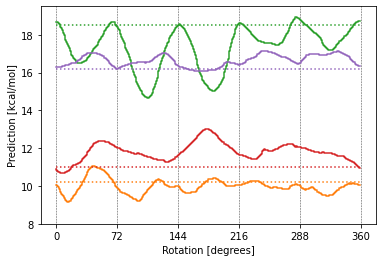
\includegraphics[width=1.0\textwidth]{figures/regression/snap/aug-5steps-30per.png}
  \endminipage\hfill
  \minipage{0.5\textwidth}
  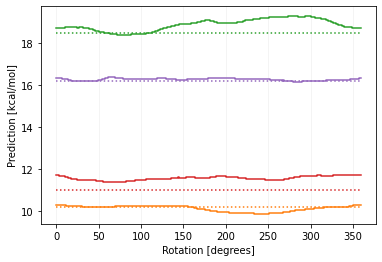
\includegraphics[width=1.0\textwidth]{figures/regression/snap/aug-30steps-30per.png}
  \endminipage\hfill
  %\hfill  
  %\minipage{0.3333\textwidth}
  %  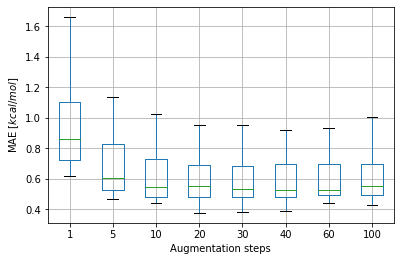
\includegraphics[width=1.0\textwidth]{figures/regression/snap/augmentation.png}
  %\endminipage\hfill
  \caption[Evaluation of SNAP rotational invariance]{
  The predictions for a network on SNAP features for $n_{max}=9, l_{max}=3$ trained with 5 data augmentation steps (left) 
  and 20 augmentation steps (right) for 4 randomly selected samples from the test dataset.
  The continuos line is the prediction of the network, the dotted line is the calculated barrier.
  The networks were trained on a train split of 70\%.
  %On the right are the results for multiple models trained on different augmentation steps.
  %All networks are trained on the same network architecture, at different train fractions.
  }
  \label{fig:snap_roation}

\end{figure}


\paragraph{Results}

With the data learned from the extensive hyperparameter and input space exploration, a final hyperparameter
optimization was performed.
This hyperparameter optimization took into account the values discussed previously, and therefore was run on 
features  generated with $ n_{max} \in \{8,9\}, l_{max} \in \{3,4\}, r_{cut}=8$.
30 data augmentation steps were passed to the hyperparameter optimizer.
Hyperparameter optimization was run on a train fraction of 80\% of the dataset.
This time, the hyperparameter space was increased slightly to allow the optimizer
to choose from up to 10 hidden layers, each with a maximum amount of 1000 neurons.


\begin{figure}[!htb]
  \minipage{0.5\textwidth}
    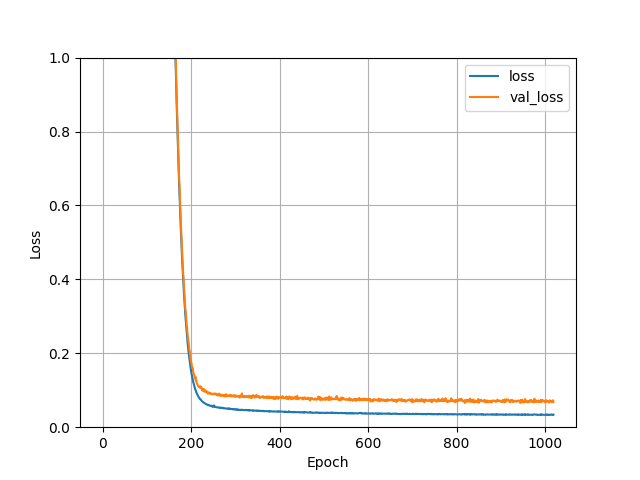
\includegraphics[width=1.0\textwidth]{figures/regression/snap/loss_8-4.png}
  \endminipage\hfill
  \minipage{0.5\textwidth}
  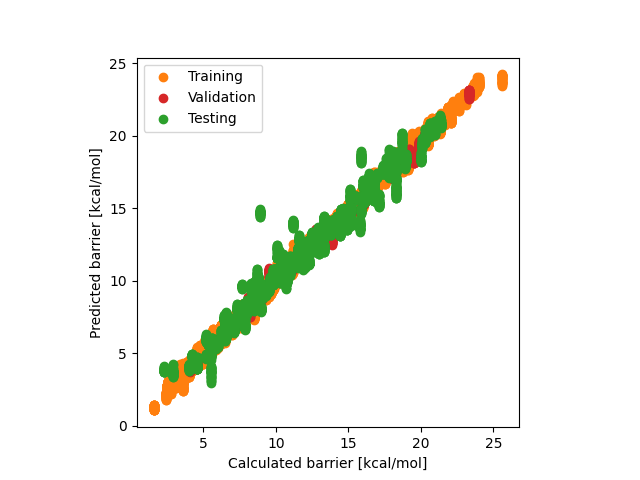
\includegraphics[width=1.0\textwidth]{figures/regression/snap/scatter_8-4.png}
  \endminipage\hfill  
  \caption[Best performing model on SNAP features]{
    Loss of the best performing model on SNAP features with  $n_{max}=8, l_{max}=4$ on the left. 
    The loss function used is mean squared error.
    Predictions of the model trained on a training fraction of 80\% on the right. 
    For every sample, 30 data augmentation steps are used. This makes some samples appear like small vertical lines.
    The model achieves an accuracy of accuracies of $0.52980 kcal/mol$ and
    $r^2 = 0.96231$.
  }
  \label{fig:snap_roation}

\end{figure}


Even with slight variations in prediction accuracy due to rotation, the overall results of regression performed on SNAP features is still promising.
All models found during hyperparameter optimization for different $n_{max}, l_{max}$ were able to predict the reaction barrier with accuracies in the
range of the best regression methods found so far.
With the best models for $n_{max}=8, l_{max}=4$ achieving accuracies of $MAE=0.530 kcal/mol$ and $r^2=0.0.962$. %TODO: Verbessern

The network has a total of 7 hidden layers.
Dropout and batch normalization layers are added in between \ref{fig:architectures}.

Compared to other modes of encoding the data, SNAP seems to be especially susceptible to outliers.
For all models, the regression accuracy is heavily influenced by a small number of samples with poor precision.
Since the split between training and test data is random, the overall accuracy of the model is 
heavily influenced by the selection of samples in the test data.
The same holds true for the randomness between training and validation data.

Improving the networks stability to outliers could further increase regression accuracy.


\section{Comparison}
\label{sec:Evaluation:Comparison}

The neural networks proposed here were able to predict the activation barriers with high accuracies.
The reference values to the networks was given by \cite{friederich_dos}, where different Machine Learning 
approaches to the regression problem were introduced.
While the dataset was the same in \cite{friederich_dos}, the features extracted from the molecules were different.
The comparison of the results from \citetitle*{friederich_dos} and this thesis is therefore more 
a comparison of feature extractors, and not a comparison of machine learning methods or network architectures.

Their best neural network trained on 80\% of the data achieved a prediction accuracy of $MAE = 1.12 kcal/mol$ and a 
coefficient of determination of $r^2 = 0.845$.
The neural network was 4 layers deep and trained on their autocorrelation features.
Autocorrelation features extract features based on chemical properties of an element, but neglect the 
3D structure of the molecule \cite{friederich_dos}.
The best prediction accuracy was however in a yet unreleased paper by  a graph convolution neural network (GNN) on 
a graph structure of the molecule.
It achieved an accuracy of $MAE = 0.571 kcal/mol$ and $r^2=0.964$.
These are the highest accuracies achieved on this dataset yet.
While this was the state-of-the-art  to compare the models in this thesis to, the main objective was not to beat these numbers.
The goal was rather to achieve similar performance with a feature descriptor that allowed for a mapping back from feature space to 3D space.
This allows for an extensive interpretation of the results, which is impossible with current features.
The SNAP features however not only allow for this analysis, but are also able to beat the accuracy of GNN models.
Another important metric is the performance of the networks for different sizes of training data.
The models performance will therefore be compared by their accuracy for different test split sizes.
\\
The first approach regression was using LEFD features.
When training on 80\% of LEFD features, the best neural network achieved an accuracy of $MAE = 1.096 kcal/mol$ and $r^2=0.882$.
While the accuracy is slightly higher than the best neural network in \cite{friederich_dos}, it still falls short 
of both the GNN and other machine learning models.
At lower train fractions the accuracy decreases faster than other methods.
Interestingly, the accuracy of the model is very similar to the accuracy achieved by the neural network trained on autocorrelation 
features.
Additionally the autocorrelation features could be approximated from the LEFD features reasonably well.
This could indicate that LEFD features and autocorrelation features describe
similar or correlating information about the element.
\\
The best model trained on SNAP features was able to achieve accuracies of $0.52980 kcal/mol$ and
$r^2 = 0.96231$ when trained on 80\% of the data.
This model used SNAP features with $n_{max}=8, l_{max}=4$.

While the accuracies are heavily dominated by outliers, models trained on SNAP features were consistently
able to achieve accuracies better than the best models trained on other features.
Another interesting property of models trained on SNAP is their ability to perform well with small amounts 
of training data.
Even with training fractions well below 50\% of the data, the network still achieved good accuracies.
At train fractions below $10\%$ the accuracy drastically decreases.

The biggest problem with SNAP features so far seems to be their sensitivity to outliers.
While the majority of the elements in the dataset is predicted with very high accuracy, 
there are some outlier with very poor performance.
Depending on the application of the network, a network with a lower overall accuracy 
that is less susceptible to outliers might be better suited.

\begin{figure}[!htb]
  \minipage{0.5\textwidth}
    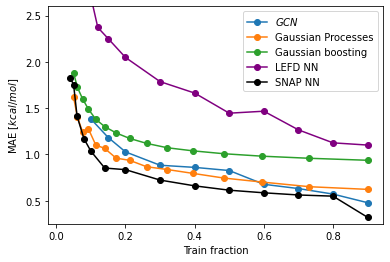
\includegraphics[width=1.0\textwidth]{figures/regression/mae-compare.png}
  \endminipage\hfill
  \minipage{0.5\textwidth}
  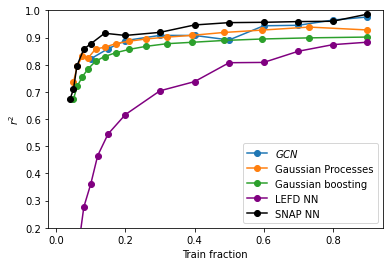
\includegraphics[width=1.0\textwidth]{figures/regression/r2-compare.png}
  \endminipage\hfill  
  \caption[Comparison of learning curves]{
    Learning curves of different machine learning methods on the same dataset.
    Gaussian Process and Gaussian Boosting models were proposed in \cite{friederich_dos}.
    The GCN is a unpublished result by \citeauthor{friederich_dos}.
  }
  \label{fig:snap_roation}

\end{figure}



\section{Explaining the prediction}

Traditionally neural networks are seen as a black-box approach to data analysis.
The network is given a set of training data and trained to fit onto the data,
the internals of the network however are set by the optimization algorithm.

This makes it hard to interpret the origin of predictions of the network.
Network explaining methods aim to help to understand the origin of a prediction in the features.
Translating the features back into chemical space can help to better understand 
the elements in the dataset and might give intuitions on how elements have to be adapted in order to change their activation barrier.

Since SNAP features achieved significantly higher prediction accuracies,
this analysis was focused on SNAP features only.

\subsection{SHAP}

The first approach to explaining the feature space was using the SHAP feature explainer.
SHAP offers analysis of the influence of different features to the final prediction \cite{NIPS2017_7062}.
This allows get an intuition on how different species influence the activation barrier.

When using SHAP values on the model, the contribution of each feature to the current prediction can be observed.
The values generated by SHAP are a matrix the size of the input to the network.
Summing over all SHAP values for one sample will give the prediction of that sample.
When labels for the features are  known, SHAP is often visualized as features pushing in opposite direction with different force 
to achieve the prediction of the model.
The SHAP values will not correspond to the activation barrier directly,
but rather to the scaled activation barrier used to train the network.

Scaling issues make the interpretation of the SHAP values difficult.
Looking back at the main objectives of SNAP, one of the main objectives was the ability to scale the features bach into 3D space.
While the formula describing the density space could be can to transform the SHAP values 
into a 3D density, it is unclear how the density generated by SHAP would have to be interpreted.

Due to the nature of the SNAP encoder, a negative $c_{nlm}^Z$ values does not automatically 
describe a negative density.
This means a negative SHAP values for an element does not equate reduction in density
at a point in space.
In order to get information about the 3D space surrounding the atom, the SHAP values would have to be converted back into 3D density space.
This is a problem since the features indicate their influence on the prediction, but do not necessarily correspond 
to the 3D spacial encoding.
The SHAP values therefore are in the scale of the activation barrier.
When converting SHAP values back to 3D, it is unclear how these scaling issues would 
affect the result. 
This uncertainty prohibits a interpretation of the density space.
Examining the density space for it's influence on the prediction is only possible if the scaling
issues can be resolved.
Since the scaling issues did not seem to be easily solvable, a second attempt to explain the origin of the prediction
was run using a gradient based method.

The information that can be extracted from SHAP values therefore is limited to feature space.

In the case of Figure~\ref{fig:shap}, the features corresponding to bromine and arsenic seem to decrease the barrier.
Interestingly the features encoding the absence of phosphorus seem to increase the barrier.

A good sign that the values have some validity is that Iridium never influences the barrier.
Since iridium is present exactly once in all elements, it should not carry any information about the barrier,
and therefore not influence the prediction at all.

SHAP allows to get some intuition of the element and how it is atoms influence the barrier.
However for now the information we can gain is limited to a global representation of the element.

If the scaling issues can be resolved, SHAP might offer further and detailed insight into how different parts of an element influence it's activation barrier.

\begin{figure}
    \centering
    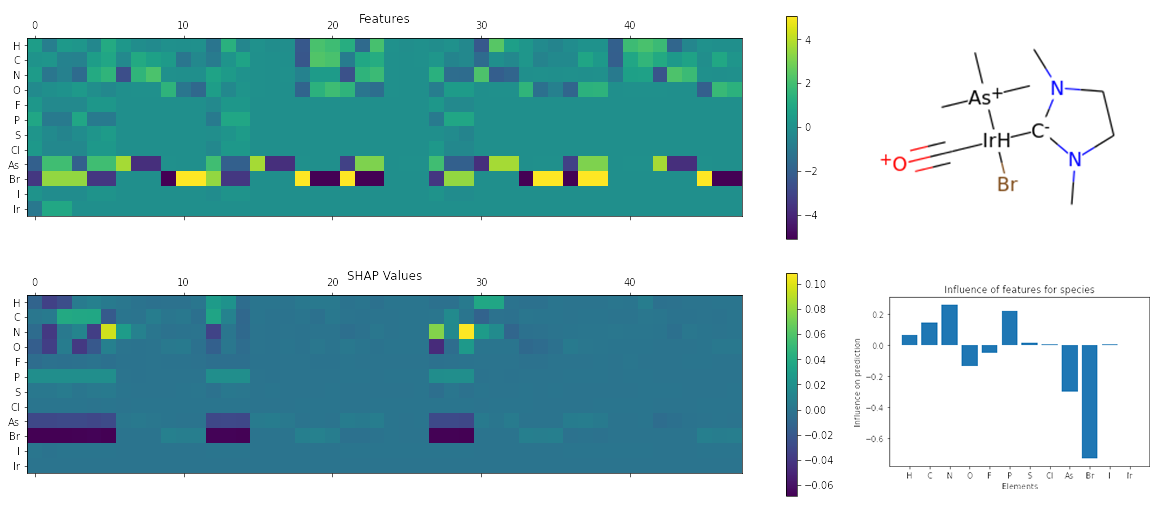
\includegraphics[width=0.9\textwidth]{figures/evaluation/SHAP.png}
    \caption[SHAP values]{
        Features($n_{max}=l_{max}=3, r_{cut}=12$) generated by the element on the right and the corresponding SHAP values.
        The element has a calculated barrier of $10.2 kcal/mol$ and was taken from the test set.
        Because the activation barriers are scaled to achieve higher prediction accuracies,
        the value the network predicts is $-0.494$. Scaled back this results in a predicted activation 
        barrier of $9.83 kcal/mol$.
     }
    \label{fig:shap}
  \end{figure}
  



\subsection{Gradient explainer}

One of the interesting properties of neural networks predicting the activation barrier from the 3D shape is 
that an intuition on how changes in 3D space will influence the activation barrier can be gained.

In contrast to SHAP values that explain the contribution of a features to the prediction of a model, 
computing the gradient of a model will give an idea on how changing a certain feature will affect the prediction of the model.

Let the model $N$ be a function from feature space $\mathbb{R}^n =: \mathbb{S}$ to the activation barrier of the element $\mathbb{R}^+_0$.
Since a function from chemical space $\mathbb{D}$ to feature space $\mathbb{S}$ can be defined,
a mapping from chemical space to the activation barrier can be found.
$$ \Psi : \mathbb{D} \to \mathbb{S} \to \mathbb{R}^+_0, e \mapsto \Psi(e) $$

While this mapping is only an approximation, the previous chapters show that the 
the accuracy of the approximation in this direction is high.

Looking at the derivative of $\Psi$, the gradient $\nabla \Psi$ points towards the steepest ascent of the activation barrier.

If $\mathbb{D} \to \mathbb{S}$ was a perfect bi-directional mapping, in theory following the gradient until a local minima is reached,
an then translate back to chemical space would mean finding an element with similar structure but a lower activation barrier.
This theoretical approach is not possible in practice.
The first problem is the networks lack of understanding of the chemical space.
A simple gradient-decent approach will therefore quickly result in illegal configurations 
that are physically not possible.
The second problem is the low resolution of the feature space.
As shown before, in many cases the density encoding a single atom will not correspond perfectly to the location of this atom.
This problem becomes even more severe when multiple atoms for one species need to be encoded.
This means a reconstruction of the molecule from density space is often impossible.

Due to the limited resolution, looking at the gradient itself is more valuable.
Instead of performing a gradient descent approach, the idea is to look at a single example of a catalyst and compute the gradient for its encoding.
When looking at the gradient, it is expected that molecules known to increase the barrier will generate a high density in the gradient.
Molecules known to decrease the barrier should generate a sub-zero density.
This would indicate that removing elements generating a high density will decrease the barrier,
while removing elements creating a negative density will increase the barrier. %TODO: Stimmt das so????

Since the gradient is determined by calculating the derivative of the the network $N$ with input $c$ in respect to the output $N(c): \mathbb{R^N} \to \mathbb{R}$
the gradient vector gives us the direction of steepest ascent for a single sample.
$$
\nabla N: \mathbb{R}^n  \to \mathbb{R}^n 
$$

Since the gradient vector is the derivative of the $c_{nlm}^Z$ coefficients, 
directly interpreting the gradient is challenging. 
Due to the nature of the SNAP encoding, negative $c_{nlm}^Z$ coefficients do not necessarily correlate to negative densities and vice versa.

Instead the difference in density when adding the gradient to the original features will be examined.
Let $f \in \mathbb{S}$ be the feature vector generated by a sample, and $g = \nabla N(f)$ its gradient.

Thinking back to the SOAP descriptor, now the density $\rho^Z(r)$ for $f$ and $f + g$ in 3D space can be computed.
The difference between these two densities should contain information about where in space density has negative or positive effects on the prediction.

$$ \rho^Z_\nabla = \rho^Z_{f+g} -  \rho^Z_{f} $$

This gives a 3D dimensional density space in which interpretations of the result can be performed.
\begin{figure}
  \centering
  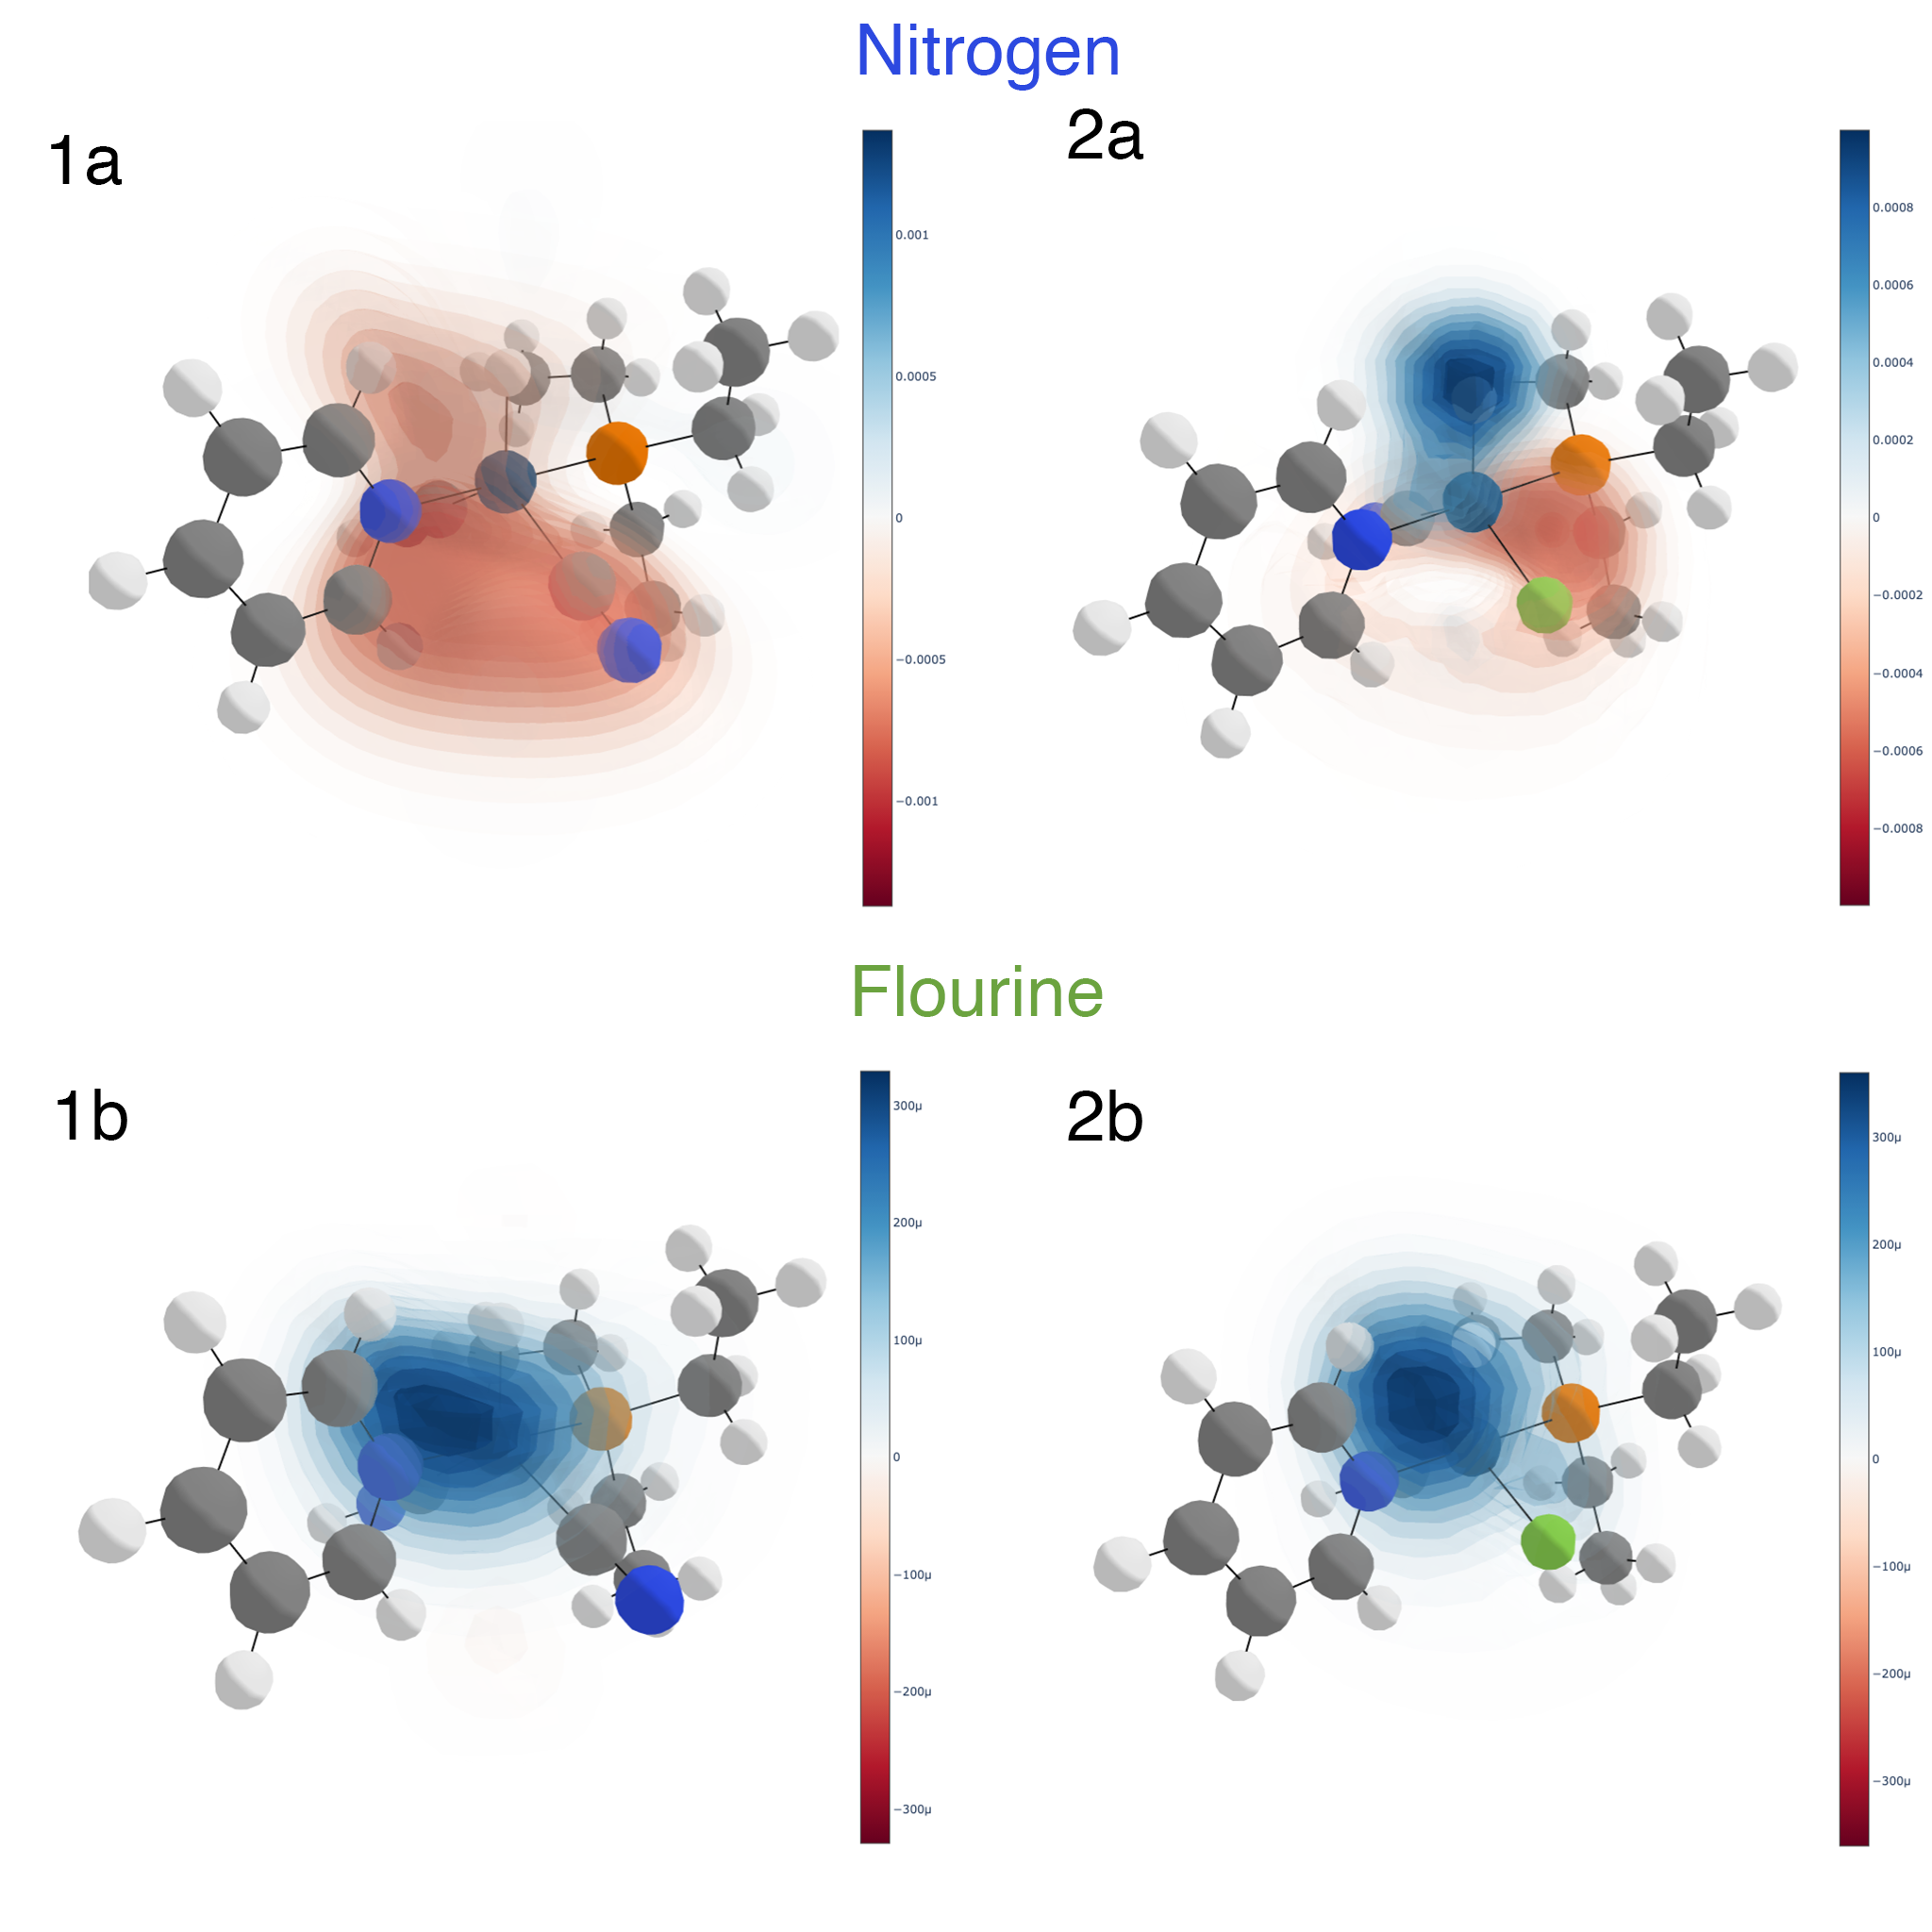
\includegraphics[width=0.9\textwidth]{figures/evaluation/GradientComp.png}
  \caption[Comparison of local gradients]{
      Gradient of a model trained on features with $n_{max}=8, l_{max}=4$ translated into 3D space.
      The element on the left has an activation barrier of $3.6 kcal/mol$, while the element on that right
      has an activation barrier of $18.0 kcal/mol$.
      The chemical structures of the molecules are identical except for the nitrogen(blue) arm of the element
      on the left being exchanged for a fluorine(green) arm for the molecule on the right.
      On the top, the gradient for nitrogen is plotted. On the bottom, the gradient for fluorine is plotted.
      More angles for plot 1a can be found in Figure~\ref{fig:gradient-sides}.
      Keep in mind that the scales for nitrogen and fluorine are different.
   }
  \label{fig:snap-gradient}
\end{figure}

Here the encoding limitations introduced earlier are encountered.
For some atoms, the encoding seems to work as expected, producing regions of negative gradient density where
an increase in the activation barrier is expected, for others the distribution is not precise enough for detailed analysis.
Looking at Figure~\ref{fig:snap-gradient}, an area of negative density for the nitrogen plot 1a of element 1 can be observed.
The negativity is relatively strong in comparison with the gradient density for other elements.
This indicates that decreasing the amount of nitrogen atoms should increase the activation barrier.
This is confirmed by the data.
When exchanging one nitrogen atom for fluorine, the activation barrier increases from $3.6 kcal/mol$ to $18.0kcal/mol$.
However, when looking at the other plots, the density plot becomes less clear.
Since the addition of the fluorine atom increased the activation barrier, the expectation is that a region of strong positive
density is indicated around the fluorine atom.
While there is a region of positive density in the plot 2b, it is way off from the fluorine atom.
Also, the density is less by about a factor 3 compared to the density of the nitrogen plot.
This would indicate adding fluorine in this region will further increase the barrier.
However adding more fluorine atoms in this region is chemically impossible. %TODO: Is it?
\\

It remains unclear what the proper interpretation of the 3D gradient density should be.
While there could be some correlation between the gradient and the actual regions where density has to be added or
removed to alter the activation barrier, differentiating between actual insight of the chemical properties and artifacts 
of the mapping between feature space and activation barrier seems challenging.

In general, the detail of the encoding does not seem high enough for localized spacial interpretation of the gradient.
Possible solutions to the resolution problem could include dramatically increasing the number of coefficients used to describe a single sample.
This comes with its own set of challenges, since the size of the features does not scale linear, but rather in $\mathcal{O}(n_{max} \cdot {l_{max}}^3)$.
The cubic scale of $l_{max}$ implies a dramatic increase in the size of the feature vector, increasing computation time for booth feature generation and training of the regression model.
\\

While the local encoding does not seem the be accurate enough for detailed interpretation,
when integrating over the entire density space, an insight about the global influence for each species can be gained.
The output looks similar to what was achieved with SHAP values, but in this case insight on how changing the density for a certain species will affect the activation barrier should be gained.
This means a high density of one species should indicate that adding more density of this species will increase the barrier.
Similarly, a low density should indicate indicate that adding more density for this species will decreased the barrier. %TODO: So rum richtig??

For easier computation, instead of an integration the sum over a grid will be computed: 

$$ \rho_\nabla^Z \sim \sum_{\mathbb{R}^3} \rho_\nabla^Z $$

When looking at the sum over $\rho^Z_\nabla$, the plot is heavily dominated by hydrogen and carbon
in many cases.
Since hydrogen and carbon are used in a variety of different ligands, the interpretability
these elements is low.
For other elements, the gradient density might be a better indication 


\begin{figure}[!htb]
  \minipage{0.5\textwidth}
    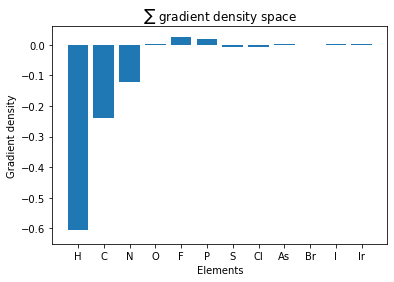
\includegraphics[width=1.0\textwidth]{figures/evaluation/elem2-GRAD.png}
  \endminipage\hfill
  \minipage{0.5\textwidth}
    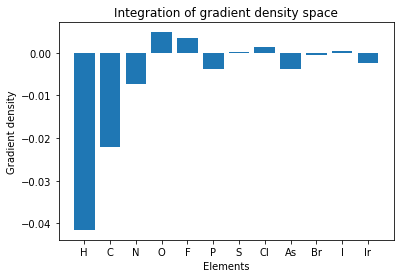
\includegraphics[width=1.0\textwidth]{figures/evaluation/elem1-GRAD.png}
  \endminipage\hfill
  \caption[Comparison of summed gradients]{
    Comparison of the gradient for molecule 1 (left) and 2 (right) for different species of atoms.
  }
  \label{fig:snap_global_gradient}

\end{figure}


It is unclear if the the chemical interpretation here should be that hydrogen and carbon play a bigger role in the activation
barrier than what was expected, or if this is an artifact of the neural network or the training data, and does not actually translate back into 
the physical world.

For other elements, the gradient behaves more like what is expected.
Looking at the nitrogen density for element 1, nitrogen has a strong negative density [Figure~\ref{fig:snap_global_gradient}].
This would indicate that decreasing the amount of nitrogen in the element should increase the activation barrier.
Looking at the second element, further increasing the fluorine density should further increase the activation barrier.
Both are consistent with the calculated barriers.

For other elements, the interpretation of the gradient becomes less clear.
In some cases, the gradient does not seem to correspond to the intuition about a molecule.
The gradient also varies between models trained on different $n_{max}$ and $l_{max}$ [Figure~\ref{fig:snap-gradient-model}].

\begin{figure}
  \centering
  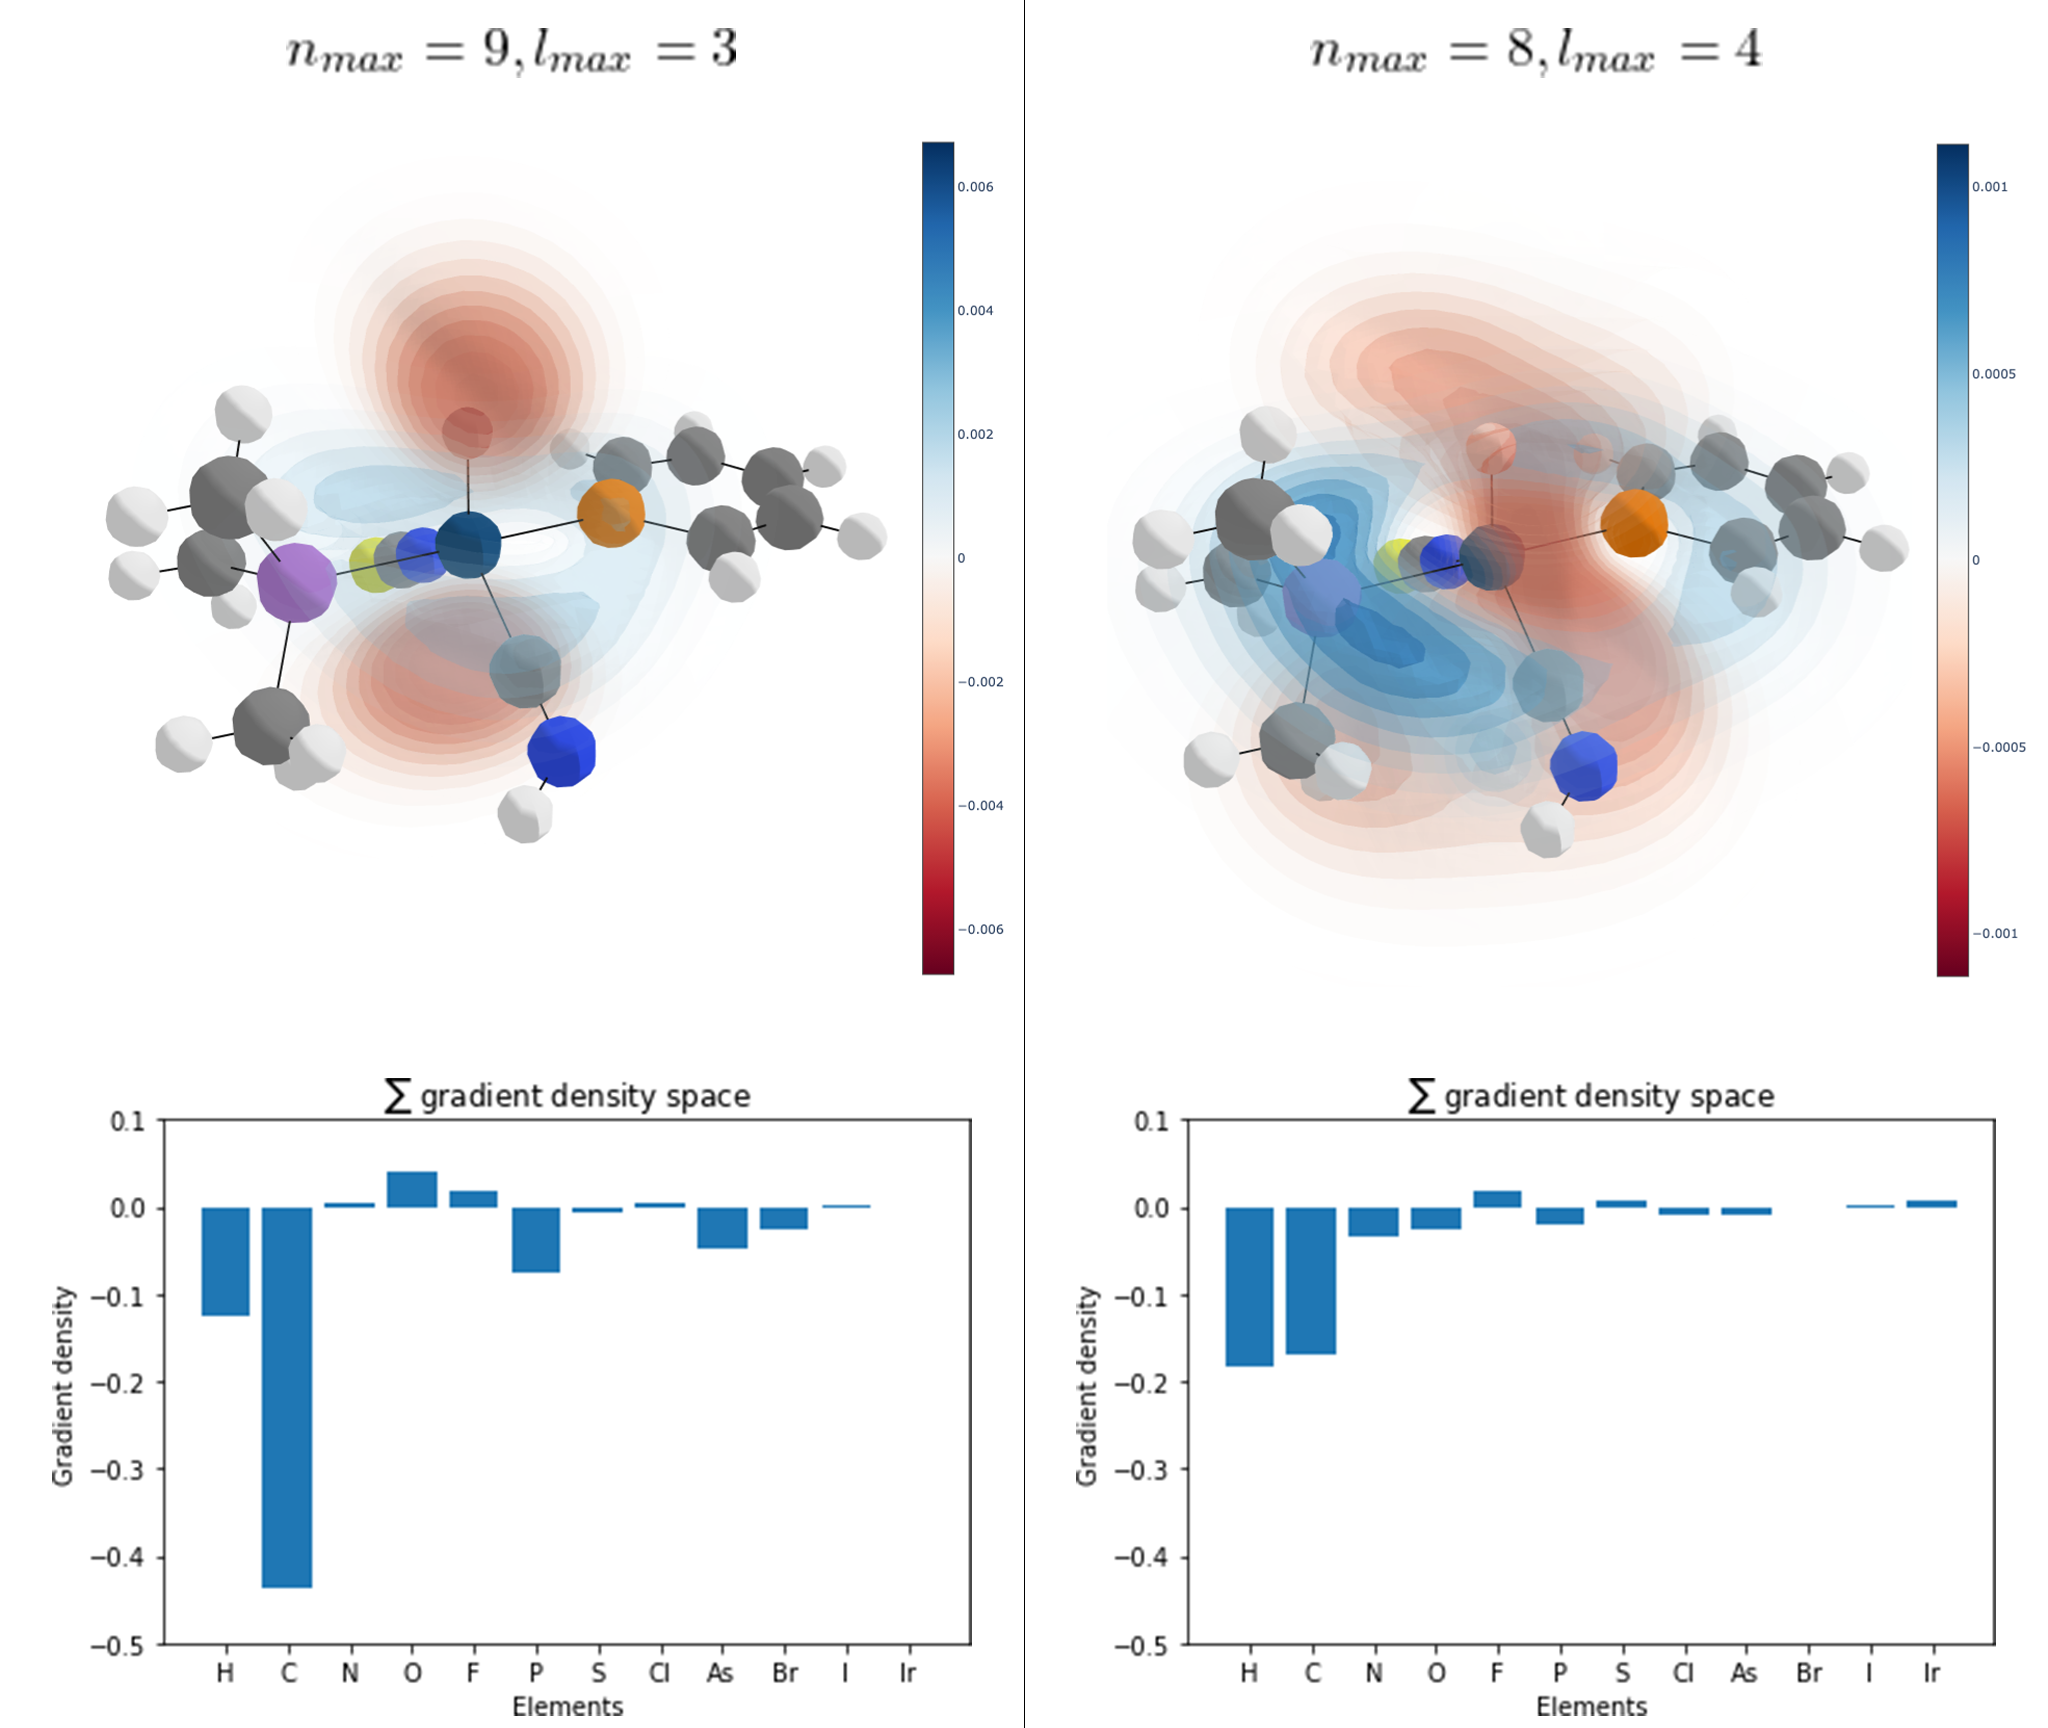
\includegraphics[width=0.9\textwidth]{figures/evaluation/Gradient-model-comp.png}
  \caption[Comparison of gradients between different models]{
      Gradient for nitrogen for the same element on 2 different models.
      The model on the left was trained on $n_{max} = 9, l_{max}=3$ while the model on the right was trained on 
      $n_{max}=8, l_{max}=4$. 
      While the shape of the 2 densities has some similarities, the scale of the density differs by a factor of 6.
      The summation over the density space has some similarities, however for some elements the difference is significant.
   }
  \label{fig:snap-gradient-model}
\end{figure}

All these uncertainties make a general conclusion about the relevance of the gradient difficult.
While there seems to be some correlation between what is expected from the gradient and what 
the data suggests, in many cases the data seems to be unclear or contradict what the chemical intuition would be.

To use the gradient for a better chemical understanding, the networks would have to undergo a more in depth analysis.
This could include an extended dataset or a higher resolution of the feature space.

For now, the SHAP values seem to offer a better insight in how chemical properties influence the activation barrier of a catalyst.
For localized interpretability, the results of gradient methods seem more promising.
While these methods show that generally an intuition about the chemical space might be learned from neural networks,
to improve the interpretability the resolution of the encoding needs to be increased further.